\documentclass[utf8, seminar, numeric]{fer}
\usepackage{booktabs}
\usepackage{csquotes}
\usepackage{url}
\usepackage{algpseudocode}
\usepackage{algorithm}
\usepackage{pgfplots}
\pgfplotsset{compat=1.15}

\algnewcommand\algorithmicforeach{\textbf{for each}}
\algdef{S}[FOR]{ForEach}[1]{\algorithmicforeach\ #1\ \algorithmicdo}

\begin{document}

\nocite{*}

\title{Problem raspoređivanja testova \\ \large{Dokumentacija}}

\author{Filip Gulan \and Jan Kelemen}

\maketitle

\tableofcontents

\chapter{Opis problema}
Problem raspoređivanja testova je vrsta problema raspoređivanja čiji je cilj rasporediti unaprijed poznati skup zadataka nad unaprijed poznatim skupom resursa uz što kraće vremensko trajanje uz poštivanje određenih ograničenja. 

Općenito ograničenja mogu biti čvrsta i meka. Čvrsta ograničenja su ona koja moraju biti zadovoljena da bi rješenje problema bilo valjano. Meka ograničenja su ona za koja je poželjno da budu zadovoljena. Prihvatljivost mekih ograničenja ne utječe na valjanost rješenja već na njegovu kvalitetu.

Kod problema raspoređivanja kvaliteta rješenja je određena tako da vrijeme trajanja izvođenja zadataka bude što kraće uz što veću količinu zadovoljenih mekih ograničenja \cite{cupicm}.

\section{Problem raspoređivanja testova}

Cilj ovog projekta je rasporediti unaprijed poznat skup testova u što kraćem vremenskom trajanju. Pojedinačni test ima svoje određeno trajanje. Vremensko trajanje je definirano kao razlika između početka izvođenja najranijeg testa i vremena završetka testa koji zadnji završava.

Uz kriterij da vremensko trajanje bude što kraće, postoje još dva ograničenja.
Pojedinačni test ima zadan niz strojeva na kojim se može izvoditi, te niz globalnih resursa koji su nužni za izvođenje testa. Oba navedena ograničenja su tvrda ograničenja.

\chapter{Opis primjenjenog algoritma}

Za probleme raspoređivanja može se primijeniti nekoliko načina rješavanja: slijedne metode, metode grupiranja, pristupi temeljeni na ograničenjima i meta-heurističke metode \cite{cupicm}. Na projektu je korištena meta-heuristička metoda, odnosno, eliminacijski \engl{steady-state} genetski algoritam. Kod genetskog algoritma se razlikuju dva pristupa: eliminacijski i generacijski.

\paragraph{Eliminacijski \engl{steady-state} genetski algoritam} uzima određen broj jedinki iz populacije, uz dani kriterij, eliminira ih te ih nadokanđuje novima dobivenim operacijama križanja i mutacije.

\paragraph{Generacijski \engl{generational} genetski algoritam} uzima određen broj jedinki iz populacije, uz dani kriterij, te od njih operacijama križanja i mutacije stvara potpuno novu populaciju.

Za genetski algoritam postoji nekoliko važnih karakteristika koji ga definiraju, a to su: reprezentacija rješenja, funkcija cilja i prikladnosti, stvaranje početne populacije, način odabira jedinki, kriterij zaustavljanja, operacije križanja i mutacije \cite{hmoea, cupicm}.

\section{Reprezentacija rješenja} 

Rješenje, odnosno fenotip, genetskog algoritma reprezentirano je kao skup parova $(\text{zadatak}, \text{stroj}, \text{početno vrijeme})$. Reprezentacija rješenja nad kojim se obavljaju genetički operatori, odnosno genotip, prikazan je skup parova $(\text{zadatak}, \text{stroj})$.

\section{Funkcija cilja i prikladnosti} \label{sec:fitness}

Funkcije cilja i funkcije prikladnosti dodjeljuju numeričku vrijednost pojedinom rješenju, koja govori koliko je rješenje kvalitetno \cite{hmoea}. Budući da u ovom problemu nema mekih ograničenja, funkcija cilja i funkcija prikladnosti je definirana kao ukupno trajanje rješenja.

\section{Stvaranje početne populacije} 

Početna populacija stvara se pohlepnim algoritmom. Za svaki pojedini test, u nasumičnom poretku, traži se najraniji trenutak kada on može započeti s izvršavanjem na nekom od strojeva na kojima mu je dozvoljeno izvršavanje. No osim strojeva, istovremeno se provjerava i dostupnost resursa za pojedini test, te se traži minimalno moguće vrijeme za koje bi test mogao biti obavljen na danom stroju uz zadane resurse. Prilikom pretraživanja mogućih vremenskih intervala za strojeve i resurse traži se najmanja/najveća (ovisno o korištenoj heuristici, objašnjeno u poglavlju \ref{sec:results}) moguća ``rupa'' u rasporedu za resurse i strojeve. Također, iako u skolpu ovog projekta to nije bio zahtjev, omogućeno je dodavanje brojnosti globalnih resursa, to jest postojanje više instanci istog resursa što bi moglo skratiti samo vrijeme izvođenja.

Tako proveden algoritam automatski stvara samo valjana \engl{feasible} rješenja u vidu dostupnih resursa i strojeva što uvelike olakšava kasniju implementaciju operatora križanja i mutacije. Na ovaj način preslikavanje testova na strojeve jednoznačno definira pojedino rješenje te se prije navedeni operatori vrlo lako mogu primjeniti na tablici kojoj je test ključ, a stroj vrijednost.

Pseudokod \ref{alg:greedy} prikazuje opisani algoritam za stvaranje valjanog rješenja te se u njemu se koristi nekoliko pomoćnih funkcija. Funkcija \textproc{is\_free} koja pronalazi vrijeme kada je stroj slobodan, te funkcija \textproc{are\_free} koja pronalazi vrijeme kada su svi potrebni resursi slobodni.

\begin{algorithm}[H]
	\floatname{algorithm}{Pseudokod}
	\caption{Stvaranje početnog rješenja}
	\begin{algorithmic}[1]
		\Function{generate\_solution}{$definition$}
				\State $solution \gets \{\}$
				\ForEach {$task \gets definition.tasks$}
				    \State $insertion \gets (time: int.max, machine: null)$
				    \ForEach {$mach \gets task.machines$}
				        \State $tp \gets 0$ \Comment{timepoint}
				        \While{$true$}
				            \State $machine\_t \gets$ \Call{is\_free}{$mach$, $tp$}
				            \State $resource\_t \gets$ \Call{are\_free}{$mach.resources$, $tp$}
				            \If {$machine\_t = resource\_t$}
				                \If {$machine\_t\leq insertion.time$}
				                    \State $insertion \gets (time, mach)$
				                \EndIf
				            \EndIf
				        \EndWhile
				    \EndFor
				    \State \Call{add}{$solution$, ($task$, $insertion$)}
				\EndFor
			\State \Return $solution$
		\EndFunction
	\end{algorithmic}
	\label{alg:greedy}
\end{algorithm}

\section{Kriterij zaustavljanja}

Kriterij zaustavljanja genetskog algoritma je karakteristika koja govori pod kojim uvjetima se genetski algoritam zaustavlja. On može biti na primjer maksimalan broj generacija ili trenutak kada se vrijednost funkcije prikladnosti prethodnog i trenutnog koraka razlikuje za manje od nekog praga \cite{hmoea}. Za potrebe ovog projekta korišteno je ograničenje maksimalnog broja generacija te makismalnog broja generacija bez promjene, uz dodatak vremenskog kriterija prilikom evaluacije zadanih instanci problema.

\section{Korak eliminacijskog genetskog algoritma}

Jedan korak genetskog algoritma sastoji se od odabira jedinki, operacija križanja nad odabranim jedinkama te operacija mutacije dobivenog djeteta, te zamjene jedinki iz populacije novo-dobivenim jedinkama.

\subsection{Način odabira jedinki}

Kao način odabira jedinki u ovom projektu odabrana je k-turnirska ($k > 2$) selekcija. K-turnirska selekcije je selekcija pri kojoj se iz populacije izvlači nasumičan uzorak od $k$ rješenja \cite{cupicmmeta}. Zatim se dva najbolja rješenja, od $k$ odabarnih, križaju, provodi se operacija mutacije nad dobivenim djetetom, te se tako dobiveno dijete zamijeni s najlošijom jedinkom iz $k$ odabranih, no naravno uz uvjet da je dobivena jedinka bolja od one koja se mijenja.

\subsection{Operacije križanja i mutacije}

Operacija križanja je operacija kojom se kombiniraju dva postojeća rješenja u novo rješenje. Implementirane su dvije verzije operacije križanja, nasumično križanje te križanje s $n$ točaka prekida.

\paragraph{Nasumično križanje} uzima dvije instance rješenja te za svaki test i uz određenu vjerojatnost uzima stroj pridružen testu jednoj od instanci rješenja.

\paragraph{Križanje s $n$ točaka prekida} uzima dvije instance rješenja te u $n$ točaka prekida za pojedini genotip testova uzima strojeve iz jednog rješenja pa nakon toga iz drugog rješenja naizmjence, s tim da se točke prekida odabiru nasumično.

Operacija mutacije je operacija kojom se izmjenjuje jedno rješenje. Primjenom operacije mutacije moguće je poboljšati kvalitetu tog rješenja ili ga pomaknuti iz lokalnog optimuma. Također se primjenjuje uz određeni vjerojatnosni prag. Implementirana operacija mutacije mijenja stroj na kojemu se pojedini test izvršava s jednim od mogućih strojeva za dani test.

\section{Pseudokod}

Pseudokod \ref{alg:genetic} prikazuje primijenjeni algoritam. U njemu se koristi nekoliko pomoćnih funkcija. Funkcija \textproc{k\_best\_solutions} koja vraća $k$ najboljih rješenja iz predane populacije. Funkcija \textproc{select\_random} koja vraća $k$ nasumičnih rješenja iz predane populacije. Funkcija  \textproc{worst\_solution} koja vraća najgore rješenje iz predane populacije. Funkcija \textproc{fitness} čije je ponašanje opisano u poglavlju \ref{sec:fitness}. Funkcija \textproc{swap} koja zamjenjuje predane jedinke iz populacije.

\begin{algorithm}[H]
	\floatname{algorithm}{Pseudokod}
	\caption{Eliminacijski genetski algoritam}
	\begin{algorithmic}[1]
		\Function{genetic}{$definition$, $population$, $max\_iterations$}
		    \State $iteration \gets 0$
		    \State $best\_solution \gets$ \Call{k\_best\_solutions}{$population$, $1$}
		       \While {$iteration \neq max\_iterations$}
		            \State $iteration \gets iteration + 1$
		            \State $k\_random \gets$ \Call{select\_random}{$population$, $k$}
		            \State $two\_best \gets$ \Call{k\_best\_solutions}{$k\_random$, $2$}
		            \State $child \gets$ \Call{crossover}{$two\_best$}
		            \State $child \gets$ \Call{mutate}{$child$}
		            \State $worst \gets$ \Call{worst\_solution}{$k\_random$}
		            \If {\Call{fitness}{$child$}$ \leq $\Call{fitness}{$worst$}} \State{}
		                \Call{swap}{$child$, $worst$}
		            \EndIf
		        \EndWhile \State{}
		\Return $bestSolution$
		\EndFunction
	\end{algorithmic}
	\label{alg:genetic}
\end{algorithm}

\chapter{Dobiveni rezultati}  \label{sec:results}

Sam pohlepni algoritam, odnosno heuristika, za generiranje valjanog rješenja iz niza parova $(\text{zadatak}, \text{stroj})$ nema hiperparametre te kao takva nije bila dio optimizacijskog algoritma no isprobane su razne implementacije. Kao najbolja heuristika se pokazala ona gdje su testovi raspoređivani na način da ``rupa'' između trenutnog testa i testa prije bude što veća jer na taj način će se prvo popuniti veliki odmaci između dva testa. Iduća bolja heuristika je uključivala isto ``rupe'', samo u obrnutom uvjetu u odnosu na prvu, to jest prvo bi se popunile manje rupe, zatim one veće, ali zbog mogućih ovisnosti o velikom broju resursa u većini slučajeva te velike ``rupe'' nije moguće smanjiti. Uz već navedene heuristike, također je isprobana i ona gdje su se prvo popunjavali prvi slobodni strojevi, no bila je lošija nego ostale dvije, za neke instance i znatno.

Nakon pohlepno generirane populacije gore korištenim heuristikama slijedio je genetski algoritam. Kao najbolji se pokazao eliminacijski genetski algoritam koji je koristio $3$-turnirsku selekciju. Kao najbolji operator križanja pokazalo se križanje s dvije točke prekida uz vjerojatnost mutacije $0.35$. Isproban je i generacijski genetski algoritam, no konvergirao je puno sporije u odnosu na eliminacijski te je pretraživanje često znalo jako varirati, stoga smo se u projektu posvetili eliminacijskoj inačici.

\begin{table}
\centering
\caption{Vremena za pojedine instance}
\label{table:times}
\begin{tabular}{|c|c|c|c|}
\hline
\textbf{}     & \textbf{1m} & \textbf{5m} & \textbf{30m} \\ \hline
\textbf{ts1}  & 41162       & 41162       & 41020        \\ \hline
\textbf{ts2}  & 37575       & 37437       & 37292        \\ \hline
\textbf{ts3}  & 40080       & 39841       & 39644        \\ \hline
\textbf{ts4}  & 35005       & 34857       & 34721        \\ \hline
\textbf{ts5}  & 41471       & 41210       & 41210        \\ \hline
\textbf{ts6}  & 45799       & 45799       & 45799        \\ \hline
\textbf{ts7}  & 41000       & 40541       & 40472        \\ \hline
\textbf{ts8}  & 44523       & 44523       & 44355        \\ \hline
\textbf{ts9}  & 42088       & 41778       & 41645        \\ \hline
\textbf{ts10} & 32478       & 32462       & 32181        \\ \hline
\end{tabular}
\end{table}

Najbolja dobivena rješenja uz prije opisanu heuristiku generiranja valjanog rješenja i genetski algoritam, prikazana su u tablici \ref{table:times} te na grafu \ref{fig:times}. Svaki redak tablice predstavlja jednu zadanu instancu, a svaki pojedini stupac najbolje rješenje nakon jedne minute, pet minuta i pola sata izvođenja genetskog algoritma. Također, u tablici \ref{table:evals} te na grafu \ref{fig:evals} su prikazani brojevi evaluacije funkcije cilja do danog trenutka. Kao i kod tablice \ref{table:times}, redak predstavlja jednu zadanu instancu, a svaki pojedini stupac broj evaluacija funkcije nakon jedne minute, pet minuta i pola sata izvođenja genetskog algoritma.

\begin{figure}[H]
	\centering
	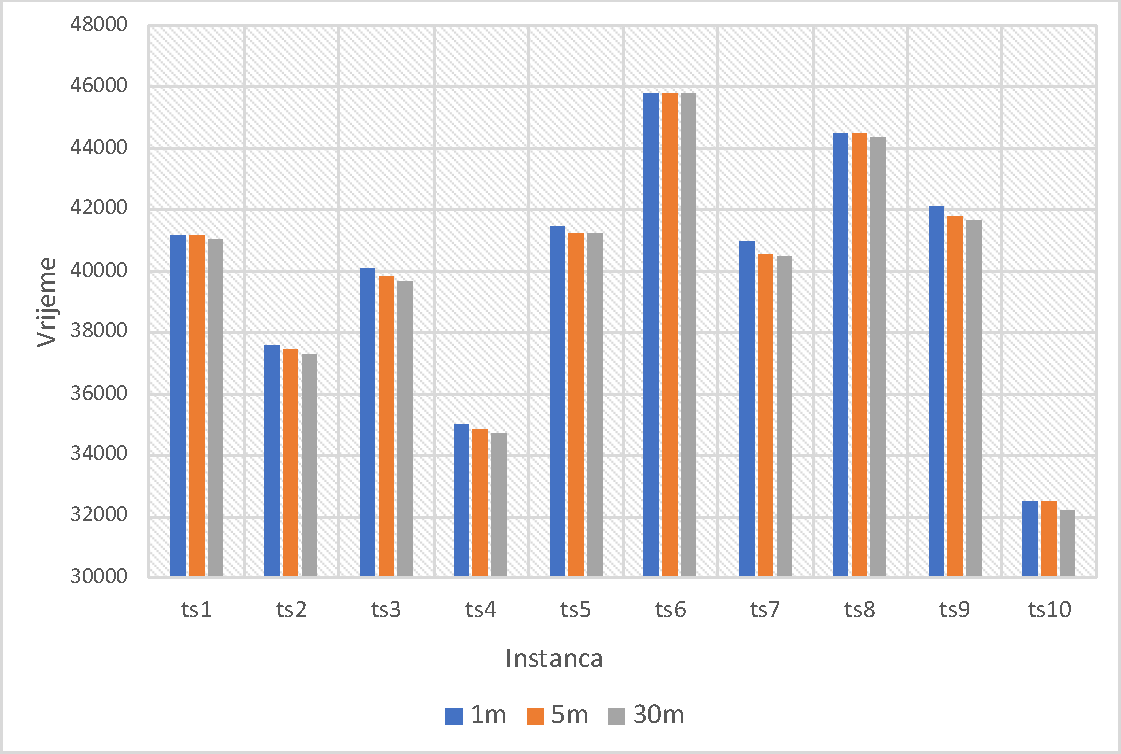
\includegraphics[width=1.0\textwidth]{times.pdf}
	\caption{Vremena za pojedine instance}
	\label{fig:times}
\end{figure}

\begin{table}
\centering
\caption{Broj evaluacija pojedine instance do danog trenutka}
\label{table:evals}
\begin{tabular}{|c|c|c|c|}
\hline
              & \textbf{1m} & \textbf{5m} & \textbf{30m} \\ \hline
\textbf{ts1}  & 27957       & 140768      & 863393       \\ \hline
\textbf{ts2}  & 30880       & 157448      & 968336       \\ \hline
\textbf{ts3}  & 28213       & 145032      & 887500       \\ \hline
\textbf{ts4}  & 32671       & 198274      & 1028706      \\ \hline
\textbf{ts5}  & 29947       & 149138      & 888751       \\ \hline
\textbf{ts6}  & 24975       & 129993      & 791991       \\ \hline
\textbf{ts7}  & 30853       & 156879      & 952876       \\ \hline
\textbf{ts8}  & 27357       & 138378      & 756266       \\ \hline
\textbf{ts9}  & 37029       & 152286      & 1118637      \\ \hline
\textbf{ts10} & 33298       & 190504      & 1194937      \\ \hline
\end{tabular}
\end{table}

\begin{figure}[H]
	\centering
	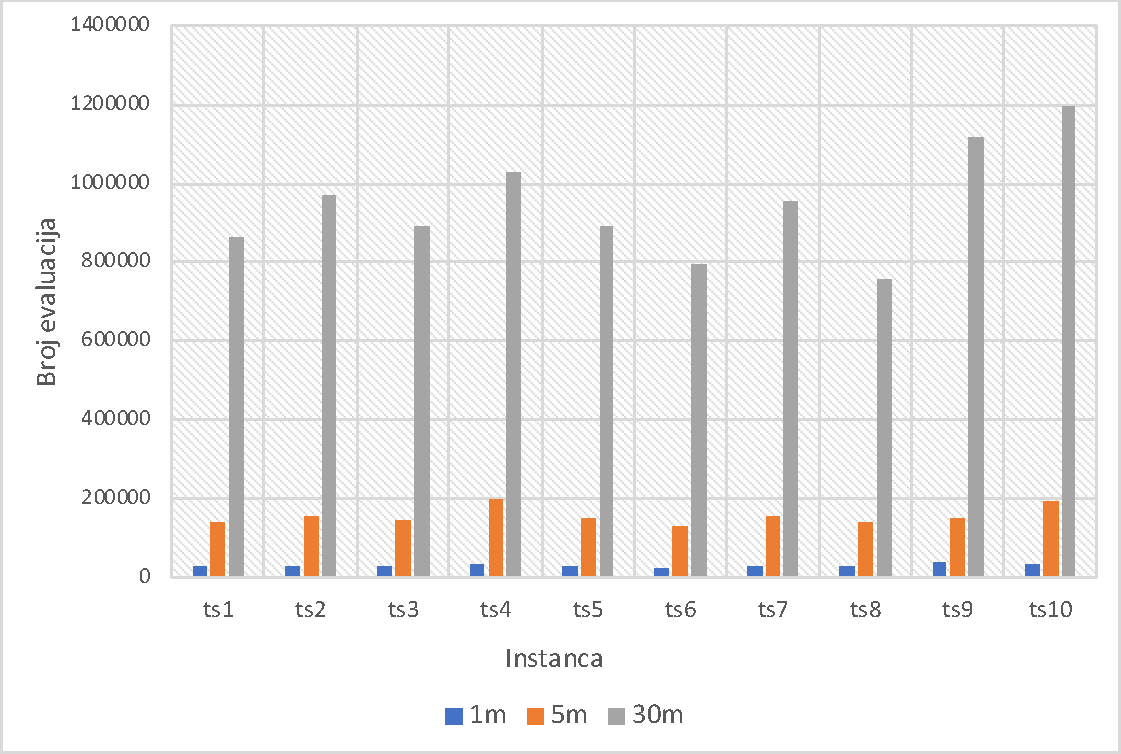
\includegraphics[width=1.0\textwidth]{evals.pdf}
	\caption{Broj evaluacija pojedine instance do danog trenutka}
	\label{fig:evals}
\end{figure}
 
\chapter{Zaključak}

Eliminacijski genetski algoritam u kombinaciji s dobrom heuristikom pri pohlepnom algoritmu se pokazao iznimno dobrim za rješavanje problema raspoređivanja testova. Sva dobivena rješenja algoritam je uspio pronaći u nekoliko minuta, i to bez paralelizacije genetskog algoritma. Sva dobivena rješenja su vrlo blizu samoj donjoj granici uzevši u obzir pojedine resurse.

Kao poboljšanja bi se mogle ukomponirati prije opisane heuristike u jednu. Također, mogao bi se isprobati paralelni genetski algoritam, uz generacijsku inačicu s nešto kompleksnijim operatorima križanja. Isto tako bi se mogla isprobati nešto drugačija reprezentacija genotipa gdje bi implicitno bili uključeni i resursi.

\bibliography{literatura}
\bibliographystyle{fer}

\end{document}
